\documentclass{article}

\usepackage[german]{babel}
\usepackage[a4paper,top=2cm,bottom=2cm,left=3cm,right=3cm,marginparwidth=1.75cm]{geometry}
\usepackage{amsmath}
\usepackage{graphicx}
\usepackage[colorlinks=true, allcolors=blue]{hyperref}
\usepackage{algorithmic}
\usepackage{algorithm}
\usepackage[font=small,labelfont=bf]{caption} % Required for specifying captions to tables and figures
\usepackage{booktabs}
\usepackage{siunitx}
\bibliographystyle{plain}


\begin{document}
\begin{titlepage}
      \begin{center}
          \Huge
         % \text{Universit\"at Innsbruck} \\
          \vspace{1cm} % Add some vertical space
          
          
          
\includegraphics[width=7cm]{res/universitaet-innsbruck-logo.jpg} \\
          \Large
          Institut f\"ur Informatik \\
          \vspace{1cm}

          \Huge
          \textbf{Heuristische Optimierung der Operatorplatzierung in verteilten Stream-Verarbeitungssystemen} \\
          \vspace{3cm} % Add more vertical space

          \Large
          Cedric Immanuel Sillaber \\
          Matrikel-Nr: 12211124
          
          \vspace{1cm}
          \large
          VU Einführung in das wissenschaftliche Arbeiten \\
          Sommersemester 2024\\
          \vspace{4cm}
          \normalsize
          Betreuer:\\ Prof. Dipl.-Ing. Dr. Thomas Fahringer
          
          \vfill 
          
          \large
          \today
      \end{center}
  \end{titlepage}
\begin{abstract}
In den vergangenen Jahren wurden Big Data Applikationen stets populärer. 
Da die Anzahl der Daten umfangreicher wird, werden effiziente Ansätze für 
verteilte Stream-Datenverarbeitung (SVS) benötigt.
Ein wesentlicher Performance-Faktor dabei ist das Problem der Operatorplatzierung.
Für das Lösen dieses Problems gibt es jedoch keine 
effiziente Lösung. Diese Arbeit beschäftigt sich mit effizienten heuristischen Methoden, die die optimale Lösung approximieren. 
\end{abstract}

\section{Revision der Seminararbeit auf Basis der Gutachten}
Von Reviewer 2 gab es einige Hinweise für die Kohärenz zwischen deutschen und englischen Begriffen. 
Beispielsweis wurde in der Originalfassung Ressourcenmodell auseinander geschrieben  "Ressourcen Modell". 
Das selbe gilt für Datenstrommodell.
Zudem gab es Inkonsistenzen zwischen den Namen der Heuristiken. Die Namen wurden nach dem Hinweis auf "Tabusuche" und "Greedy First-Fit angepasst.
Zusätzlich wurde darauf hingewiesen, dass der Separator von NP-schwer und Greedy First-Fit Ansätze 
vereinheitlicht werden sollten. Dem stimme ich nicht zu. Für NP-schwer wird typischerweise ein Bnidestrich verwendet. 

Nach der Revision von Reviewer 1 wurde ein kurzer Überblick über die Struktur der Arbeit hinzugefügt. Zusätzlich wurde der Abschnitt \ref{SVS-Definition} und \ref{OPP-Definition} überarbeitet. 
Abbildung \ref{topologies} wurde vergrößert und etwas besser strukturiert. Wie Reviewer 1 angemerkt hat, war die Tabelle \ref{experiment-tabelle} etwas unverständlich. Somit wurde sie überarbeitet. 




\section{Einführung}
Im Zuge der fortschreitenden Digitalisierung hat sich die Datenverarbeitung zu einem zentralen Aspekt der modernen Welt entwickelt.
Der Erfolg vieler Unternehmen beruht auf der Fähigkeit, kontinuierlich anfallende Datenmengen effizient zu verarbeiten.
Rund um die Uhr werden Daten gesammelt, die in Echtzeit verarbeitet werden müssen. 
Verteilte Stream-Verarbeitungssysteme (SVS) sammeln, filtern und verarbeiten Daten. Die Daten stammen von einer Vielzahl an Geräten.
Derartige Systeme werden beispielsweise in der Analyse von Finanzmärkten \cite{k5}, 
Verarbeitung von sozialen Netzwerk-Interaktionen und der Beobachtung von Network-Traffic \cite{k5} 
eingesetzt. 

Ein SVS besteht aus einer Menge von unabhängiger Operatoren, die spezifische
Funktionalitäten ausführen. Diese Unabhängigkeit ermöglicht es, dass die Rechner im Netzwerk (Cloud-Edge \cite{k6}) lokalisiert werden können, 
anstatt in der Cloud.
In solch einem System stehen zahlreiche Ressourcen zur Verfügung. 
Als Operatorplatzierung bezeichnet man das Problem, 
die Operatoren im System optimal auf verfügbare Knoten zu platzieren. 
Die Lösung dieses Problems ist jedoch NP-hard \cite{cardellini-optimal_operatorplc}.

Abbildung \ref{SVS-figure} zeigt ein SVS. Eine Anzahl von Datenquellen $P$ produziert Daten, die zu den Senken $C$ geleitet werden. Die Operatoren 
werden in der Abbildung als $SBON$ bezeichnet. Das Operatorplatzierungproblem (OPP) beschäftigt sich mit der Frage, 
welche physischen Knoten die Operatoren aufnehmen sollen \cite{network-aware-op}. 

Für die Evaluation solcher Modelle werden diverse Quality-of-Service (QoS) Attribute herangezogen. 
Dazu gehören Durchsatz, Ende-zu-Ende-Latenz und Verfügbarkeit \cite{efficient-operator-placement,cardellini-optimal_operatorplc}.
 Der Ansatz in dieser Arbeit versucht sich auf generalisierte QoS-Attribute 
zu fokussieren, die einfach angepasst werden können \cite{efficient-operator-placement}.

Diese Arbeit fokussiert sich auf einen Ansatz, der bekannte Heuristiken kombiniert und das Optimum effizient approximiert. 
Der Ansatz bezieht sich auf keine spezifische SVS Implementierung und ist somit \textit{modell-frei}. Folglich kann diese Lösung für verschiedene Systeme angewendet werden.
Die optimale systematische Position in solch einem System stellt einen maßgeblichen Performance-Faktor dar. 


\begin{center}
    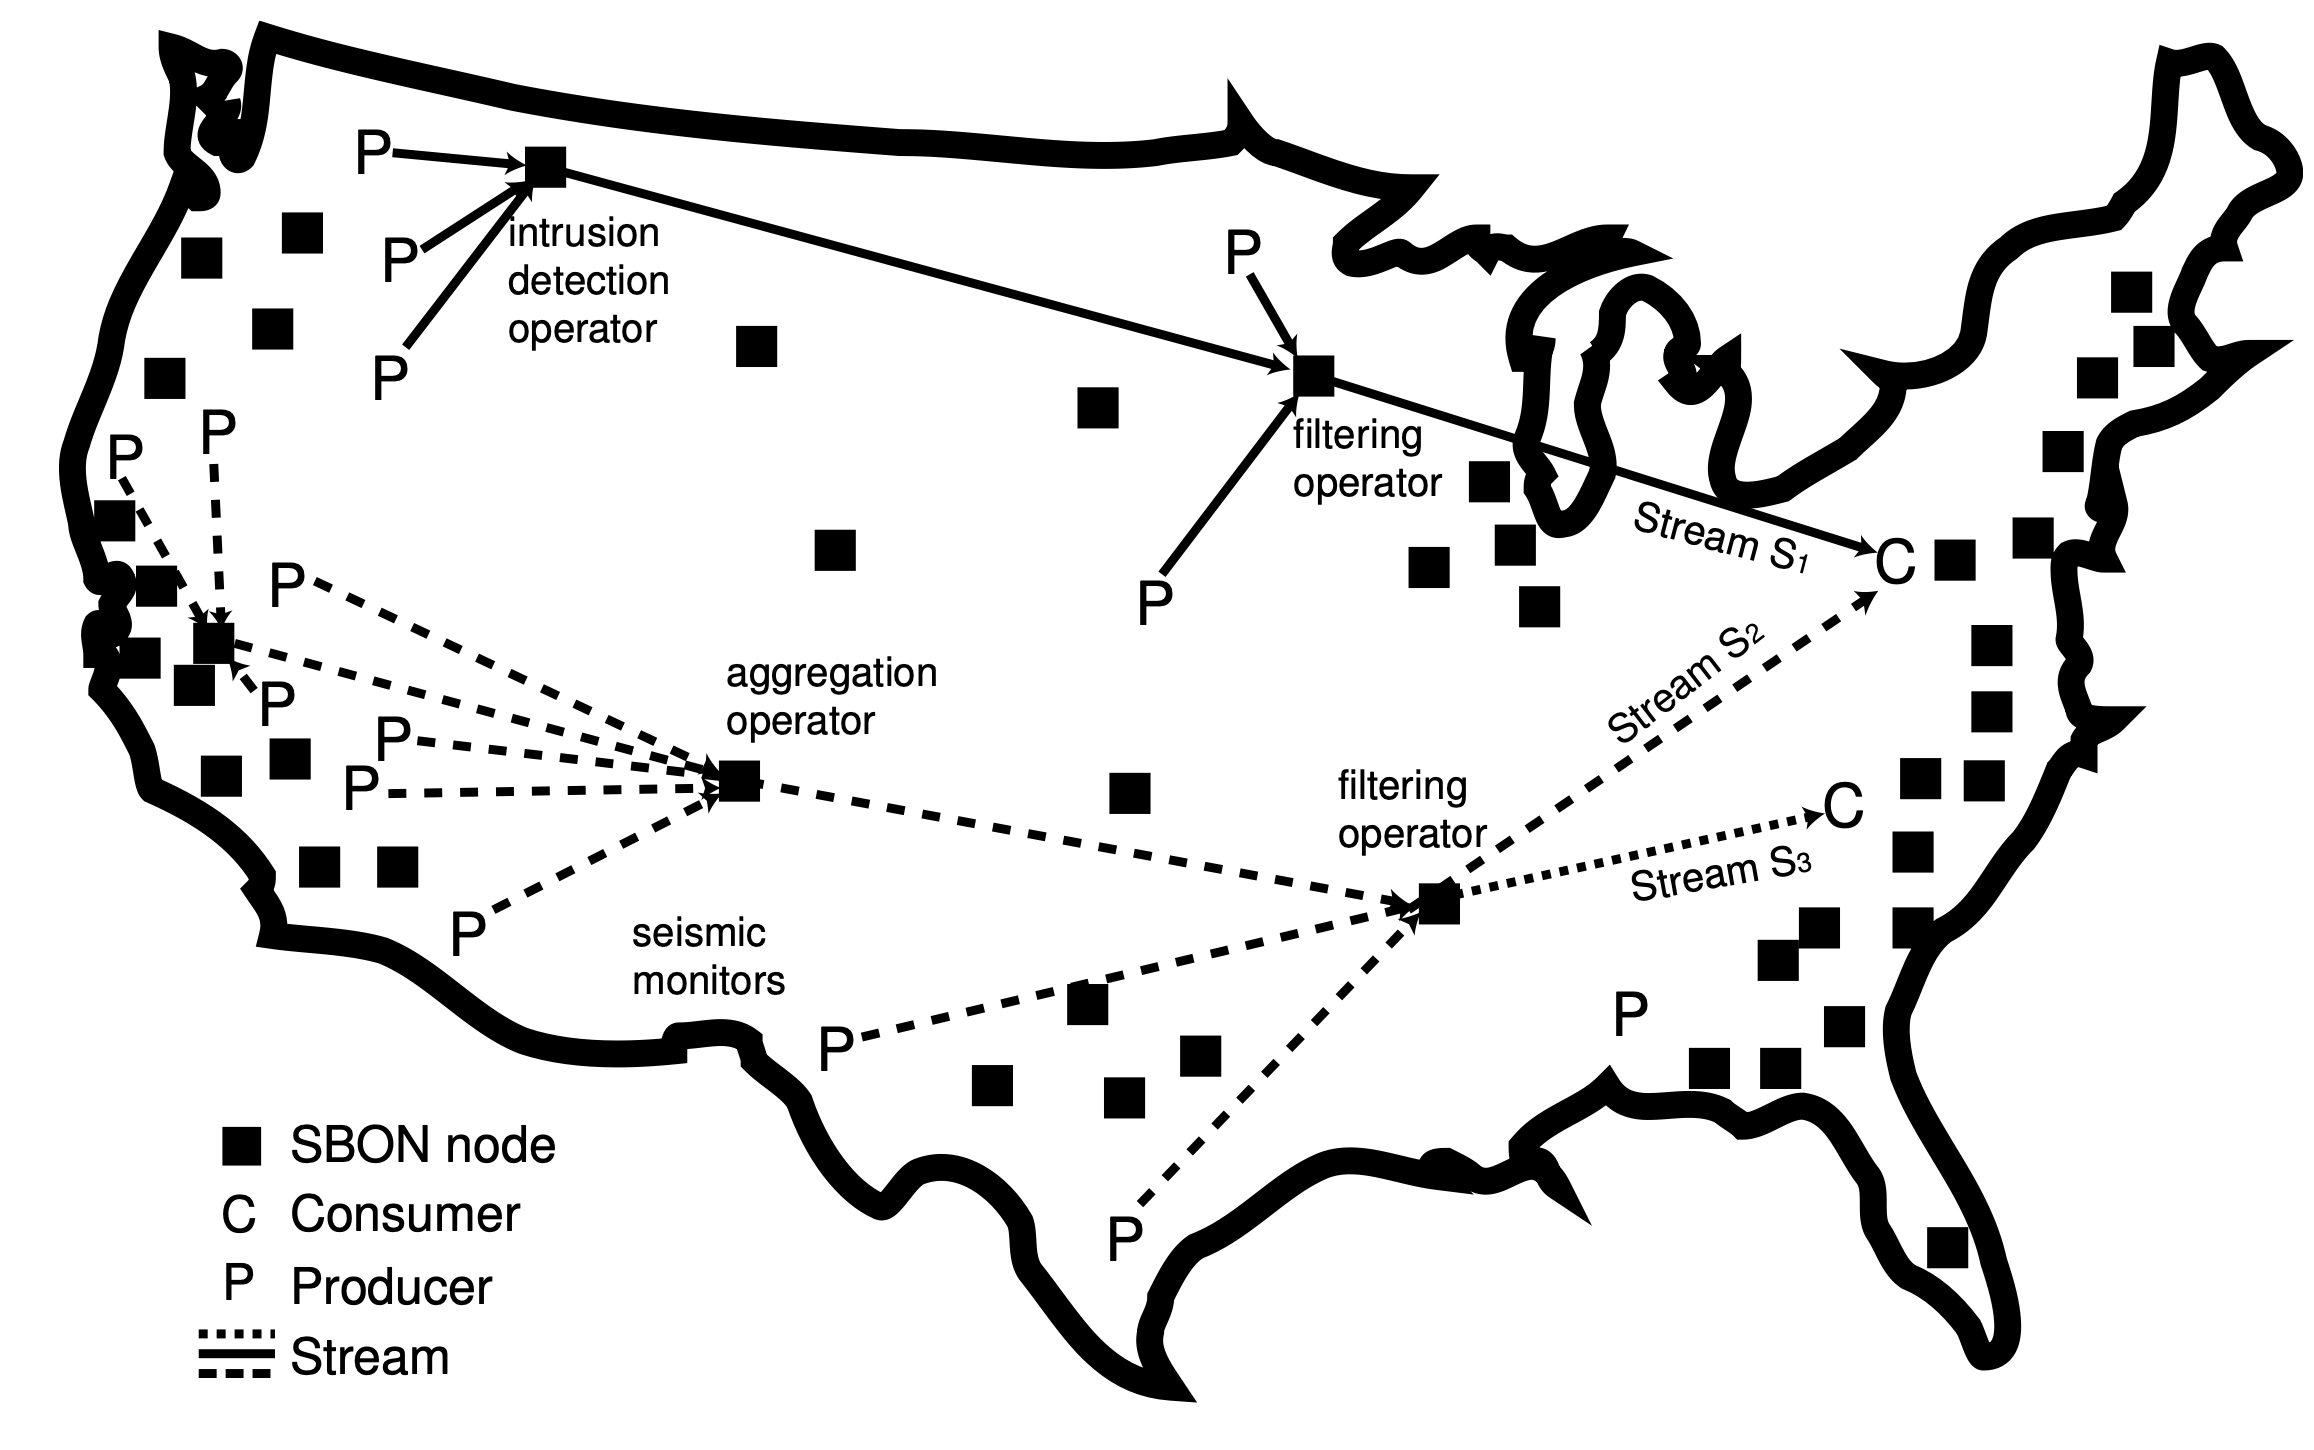
\includegraphics[width=0.5\linewidth]{res/SVS.png}
    \captionof{figure}{Stream Verarbeitungssystem, Quelle: \cite{network-aware-op}.} 
    \label{SVS-figure}
\end{center}

\textcolor{red}{Die Arbeit ist wie folgt strukturiert: In Abschnitt 3 werden verwandte Arbeiten vorgestellt. 
Darauf folgt ein Abschnitt mit den wichtigsten Definition für die Formulierung des Optimierungsproblems. Anschließend werden Heursitiken vorgestellt, die das Optimierungsproblem approximieren.  
In Abschnitt 6 werden die vorgestellten Heuristiken in einem Experiment evaluiert.}

\section{Verwandte Arbeiten}
Das Problem der Operatorplatzierung (OPP) wurde aufgrund seiner Bedeutung in der Forschung umfassend untersucht. 
In der Literatur werden verschiedene Aspekte der Operatorplatzierung beleuchtet, wie in den Arbeiten von \cite{survey-placement-strategies,Starks2018} zusammengefasst. 
Insbesondere konzentriert sich die Forschung auf drei Hauptbereiche: (1) Ziele der optimalen Platzierung, (2) unterschiedliche Optimierungstechniken, und (3) verschiedene Infrastrukturen der verteilten Systeme.
Im Hinblick auf Optimierungstechniken (Punkt 2) haben mehrere Studien verschiedene Ansätze untersucht. 
Greedy Heuristiken, wie in \cite{greedy-distr.-svs} beschrieben, bieten eine vorhersagbare und oft schnelle Lösung, die jedoch nicht immer zu optimalen Ergebnissen führt.
Ein weiterer Forschungsansatz befasst sich mit Metaheuristiken zur Optimierung des OPP. 
Arbeiten wie \cite{whiteWater} und \cite{latency-estimation-local-search} präsentieren Methoden, die auf der lokalen Suche basieren. Diese Ansätze zielen darauf ab, durch iterative Verbesserungen und das Durchsuchen des Lösungsraums bessere Platzierungsentscheidungen zu treffen.


\section{Definitionen}
Um eine konkrete Optimierung des Problems beschreiben zu können, ist es notwendig, die Problematik formal auszudrücken. 
Im Folgenden wird eine formale Abstraktion des OPP vorgestellt. 
Zuerst werden das Datenstrom- und das Ressourcenmodell \textcolor{red}{(}\ref{SVS-Definition}\textcolor{red}{)} definiert. 
Beide Modelle werden mittels Graphentheorie formuliert und beschreiben ein SVS. 
Anschließend wird das Problem der Operatorplatzierung mithilfe der zuvor definierten Modelle formuliert \textcolor{red}{(}\ref{OPP-Definition}\textcolor{red}{)}.


\subsection{Definition von SVS}  \label{SVS-Definition}  % evt "formale definition ..."
%In diesem Abschnitt werden die Grundlagen verteilter Stream-Verarbeitungssysteme eingegangen. Wir geben eine formale Darstellung SVSs und geben eine Definition für das Operatorplatzierungs Problem. Zu 
SVSs basieren auf einer Anzahl an verteilten Computer-Ressourcen, die zusammen ein komplexes System ergeben. 
Dieser Sachverhalt kann mittels Graphentheorie beschrieben werden. Grundsätzlich gibt es zwei Abstraktionen solcher Systeme. 
Erstens das \textcolor{red}{Datenstrommodell} und zweitens das \textcolor{red}{Ressourcenmodell}. 
Beide Systeme werden mit gerichteten, gewichteten zyklenfreien Graphen $G = (V,E)$ dargestellt. \\


\textcolor{red}{\textit{Datenstrommodelle}} werden durch $G_{svs} = (V_{svs}, E_{svs})$ beschrieben. 
\textcolor{red}{Hier wird der Fluss der Daten definiert}
In diesem Modell beschreiben Knoten $u \in V_{svs}$ Operatoren \textcolor{red}{, Quellen und Senken} im System. 
\textcolor{red}{Datenquellen stellen Knoten dar, die kontinuierlich Daten produzieren. Produzierte Daten werden über Operatoren verarbeitet und zu den Datenbecken geschickt. 
Datenbecken stellen den Endpunkt des Systems dar. Nachdem Daten von den verteilten Rechnern verarbeitet wurden, werden sie in den Datenbecken gespeichert.} 
Zu den Operatoren gehören auch sogenannte \textit{angepinnte} Operatoren \cite{efficient-operator-placement}, 
die Datenquellen und -becken beinhalten. Kanten $(u,v) \in E_{svs}$ beschreiben Datenverkehr
zwischen den Operatoren $u$ und $v$.  Ein Stream ist ein kontinuierliche Sequenz von Daten. \\


\textcolor{red}{\textit{Ressourcenmodelle}} werden durch den Graphen $G_{res} = (V_{res}, E_{res})$ dargestellt. 
Dabei wird der logische Zusammenschluss zwischen verfügbaren Computing Ressourcen beschrieben. Der Knoten $u \in V_{res}$ 
repräsentiert solch eine Ressource. In diesem Modell beschreiben Kanten $(u,v) \in E_{res}$ 
eine logische Verknüpfung zwischen den Rechnerressourcen $u$ und $v$.
% vielleicht Fig. 1 aus efficient operator placement hinzufügen?.


\subsubsection{Angepinnte Operatoren}
Operatoren, die fest an eine bestimmte Stelle gebunden sind, werden als \textit{angepinnte Operatoren} bezeichnet. 
Datenquellen und Datensenken sind Beispiele für angepinnte Operatoren. 
\textit{Freie Operatoren} hingegen können an beliebigen Rechnerressourcen platziert werden. Diese Operatoren befinden sich zwischen Datenquellen und Datensenken und führen 
Funktionen wie \textit{Join}, \textit{Filter} und \textit{Select} aus \cite{network-aware-op}.

In Abbildung \ref{SVS-figure} sind die mit $SBON$ bezeichneten Knoten die freien Operatoren. Diese umfassen Filter-, Aggregations- und Detektionsoperatoren.

\subsection{Problemformulierung des OPP} \label{OPP-Definition}
\textcolor{red}{Ein Operator kann aus verschiedenen Gründen nicht auf jedem Knoten im Datenstrommodell platziert werden. Diese Gründe können politischer, 
sicherheitstechnischer oder topologischer Natur sein \cite{cardellini-optimal_operatorplc}. 
Weitere mögliche Gründe sind beispielsweise technische Restriktionen oder organisatorische Vorschriften.}
Für jeden Operator $i \in V_{svs}$ gibt es eine Menge an Kandidatressourcen $V_{res}^i$ (Schreibweise wie in \cite{efficient-operator-placement}).

Das OPP kann als Zuordnungsproblem zwischen den genannten Modellen formuliert werden. 
Die Zuordnungsfunktion wird eingeschränkt, um die zu minimierenden QoS-Attribute zu berücksichtigen. 
Folglich wird der optimale Kandidat $u$ in den Kandidatenressourcen $V_{res}^i$
gesucht, damit der Operator $i$ auf Knoten $u$ platziert wird.
Hierbei bezieht sich das Problem auf die Inkonsistenz zwischen 
logisch benachbarten Operatoren im \textcolor{red}{Ressourcenmodell} $G_{res}$ und optimalen Entscheidungen der Operatoren im Datenstrom Modell $G_{svs}$.

Um das Problem formal zu definieren, verwenden wir den binären Ausdruck $x_{i,u}$ $i \in V_{svs}, u \in V_{res}: x_{i,u} = 1$ wenn Operator $i$
auf dem Rechner $u$ platziert wird, andernfalls $x_{i,u} = 0$.

\[ 
    \begin{gathered}
        \operatorname*{arg\,min}_x F(x) \\
        \sum_{i \in V_{svs}} C_i x_{i,u} < C_u \quad \forall u \in V_{res} \\ % constrain: node resource
        \sum_{u \in V_{res}^i} x_{i,u} = 1 \quad \forall i \in V_{dsp} \\ % constrain: node only placed on candidate resources
        x_{i,u} \in \{0,1\} \quad \forall i \in V_{svs}, u \in V_{res}^i
    \end{gathered}
\] 

Hierbei wird die Funktion $F(x)$ bezüglich ausgewählter QoS-Attribute minimiert. 
Dieses Multi-Objective-Optimierungsproblem wird durch die Simple Additive Weight-Technik \cite{yoon-multiple-optimization} in ein Single-Objective-Problem umgewandelt.
Für typische QoS Attribute wie Antwortzeit, Verfügbarkeit und Netzwerkverwendung \cite{efficient-operator-placement} wird die Funktion $F(x)$ wie folgt definiert:
\[ 
    \begin{gathered}
        F(x) = w_r \frac{R(x) - R_{min}}{R_{max} - R_{min}} 
        + w_a \frac{log A_{max} - log A(x)}{log A_{max} - log A_{min}} 
        + w_z \frac{Z(x) - Z_{min}}{Z_max - Z_min} 
    \end{gathered}  \label{to-miminize-function}
\] 
wo $R(x)$, $A(x)$ und $Z(x)$ die QoS-Attribute und $w_r, w_a, w_z \geq 0$ Gewichtungen sind. $R_{min}$, $R_{max}$, $A_{min}$, $A_{max}$, $Z_{min}$ und $Z_{max}$ sind die minimalen und maximalen Werte der QoS Attribute.
Es gilt $w_r + w_a + w_z = 1$.


%QoS: pplication response time Rx, the application availability A(x), and the network usage Z(x).


Mithilfe einer \textbf{Straffunktion} werden die Verbindungen zwischen zwei spezifischen Knoten bezüglich der QoS-Attribute bewertet. Dadurch wird ein Vergleich 
der Rechnerressourcen möglich. Dabei werden die Links zwischen $u \in V_{res}^i$ möglich. Auf die Straffunktion wird im Folgenden eingegangen. 




\section{Heuristiken} \label{Heurisiken}
% erwähnen dass es sich um ein model free characteristic handelt
Wie in \cite{cardellini-optimal_operatorplc} gezeigt, ist das 
OPP NP-schwer.
Da die initiale Platzierung der Operatoren ein tragender Faktor in der Performance ist, werden effiziente Heuristiken benötigt.
Unser Ansatz beinhaltet eine Kombination mehrerer bekannter Heuristiken, die die Funktion F aus \ref{to-miminize-function} minimieren. 
Eine Heuristik ist ein Verfahren, das eine schnelle Lösung für ein Problem liefert, jedoch nicht zwingend optimal ist. 

Greedy First-Fit, lokale Suche und \textcolor{red}{Tabusuche} sind dabei die gängigen Methoden. 
Greedy First-Fit Ansätze können schnell eine Lösung approximieren, jedoch sind diese nicht immer optimal. Deshalb wird er mit zur lokalen Suche erweitert.
Für Lösungen höherer Qualität wird die lokale Suche zur Tabusuche erweitert.


\subsection{Straffunktion}
% Straffunktion ist für Links, nicht für Knoten!
Die Auswahl von verschiedenen Möglichkeiten \(u \in V_{res}^i\) bringt Einbußen mit sich. Da die Daten übertragen werden müssen, kommen unvorhersehbare Netzwerklatenzen hinzu. 
Hierbei müssen Netzwerklatenz, Bandbreite und Netzwerkgeschwindigkeit \cite{efficient-operator-placement} berücksichtigt werden.
Um die Platzierungsentscheidungen zu lenken, benötigen wir eine Metrik, die die Kosten der Nutzung bestimmter Knoten/Link-Ressourcen erfasst. 
In einem idealen Szenario könnten wir alle Operatoren auf einem einzigen Knoten mit unendlicher Kapazität und Verfügbarkeit platzieren. 
Da dies in der Praxis nicht möglich ist, müssen die Operatoren auf mehrere Knoten verteilt werden, was zu Netzwerklatenzen und Netzwerkverkehr führt.
Wir führen eine Linkstraffunktion \(\delta(u, v) \in [0, 1]\) ein, die die Verschlechterung der Performance im Vergleich zur idealen Ressource misst. 
Diese Funktion ist eine gewichtete Kombination der QoS-Attribute des Links \((u, v)\) und der verbundenen Knoten \(u\) und \(v\):
\[
\delta(u, v) = w_r \delta_R(u, v) + w_a \delta_A(u, v) + w_z \delta_Z(u, v),
\]
wobei \(w_r, w_a, w_z \in [0, 1]\) die Gewichte der einzelnen QoS-Metriken sind. 
Die Terme \(\delta_R(u, v)\), \(\delta_A(u, v)\) und \(\delta_Z(u, v)\) modellieren die Strafe in Bezug auf Anwendungsantwortzeit, Verfügbarkeit und Netzwerknutzung.

Diese Strafen helfen, die Qualität und Effizienz der Ressourcenverteilung in einem verteilten System zu bewerten und zu optimieren.




\subsection{Greedy First-Fit} \label{greedy-first-fit}
Diese Heuristik wird für das Bin-Packing Problem verwendet, um eine optimale Lösung anzunähern \cite{greedy-first-fit}. 
Andere Arbeiten befassten sich schon  mit der Anwendung dieser Methode für das OPP \cite{k7, k8}.
Wir passen diese Methode an, um die Operatoren auf die verfügbaren Ressourcen zu platzieren. 
Für jeden Operator werden die verfügbaren Ressourcen $v \in V_{res}$ in einer Liste sortiert. Die Sortierung basiert auf der summierten Straffunktion $\delta$
zwischen $v$ und den angepinnten Operatoren $P$. Folglich:

\[ 
    \begin{gathered}
        u_i \in P \text{, wobei P = angepinnte Operatoren} \\
        \sum_{i=0}^{|P|} \delta(v, u)
    \end{gathered} 
\] 

Ausgewählt wird der erste Rechner in der Liste, den der Operator aufnehmen kann. Mittels Breitensuche werden für alle Operatoren Platzierungen bestimmt. 
Die daraus resultierenden Operatorplatzierungen werden als eine Konfiguration bezeichnet.

%greedy frist fit no delta beschreiben


\newpage
\subsection{Lokale Suche} \label{local-search}
Die lokale Suche ist eine iterative Heuristik zur Optimierung von Lösungen in der Nachbarschaft einer Ausgangskonfiguration. 
Dabei iteriert diese Methode über die Konfiguration, die aus der Greedy-First-Fit-Heuristik resultiert. 
Der Algorithmus \ref{local-search-algo} durchläuft drei Schritte: 
Zunächst wird eine initiale Konfiguration durch den Greedy First-Fit berechnet. 
Anschließend wird eine Nachbarschaft von ähnlichen Konfigurationen bestimmt, und schließlich wird die beste Lösung in dieser Nachbarschaft gefunden.
Um die Nachbarschaft zu bestimmen, wird zunächst eine sortierte Liste $L$ erstellt, basierend auf der Straffunktion $\delta$ wie in \ref{greedy-first-fit}.
Mit dieser Liste wird dann eine initiale Konfiguration $S$ durch den Greedy First-Fit Algorithmus erstellt (Zeile 6). \\


Solange bessere Platzierungen der Operatoren gefunden werden, iteriert die lokale Suche über die Konfigurationen  (Zeile (14)). 
Eine Verbesserung wird durch einen niedrigeren Wert der Zielfunktion $F$ definiert. 
Die Suche nach besseren Konfigurationen basiert auf den drei Funktionalitäten \textit{co-locate, swap und relocate}. \\


\begin{algorithm}[H]
    \caption{Local Search}
    \begin{algorithmic}[1]
        \STATE \textbf{function} $\mathrm{localSearch}(G_{dsp}, G_{res})$
        \STATE \textbf{Input}: $G_{\text{dsp}}$, DSP application graph
        \STATE \textbf{Input}: $G_{\text{res}}$, computing resource graph
        \STATE $P \leftarrow$ resources hosting the pinned operators of $G_{\text{dsp}}$
        \STATE $L \leftarrow$ resources of $G_{\text{res}}$, 
        sorted by the cumulative link penalty with respect to nodes in $P$
        \STATE link penalty with respect to nodes in $P$
        \STATE $S \leftarrow$  solve GreedyFirstFit($G_{\text{dsp}}$, $L$)
        \STATE \textbf{do}

        \STATE \hspace{\algorithmicindent} $F \leftarrow$  value of the objective function for $S$
        \STATE \hspace{\algorithmicindent} $S \leftarrow$  improve $S$ by co-locating operators
        \STATE \hspace{\algorithmicindent} $S \leftarrow$  improve $S$ by swapping resources
        \STATE \hspace{\algorithmicindent} $S \leftarrow$  improve $S$ by relocating a single operator
        \STATE \hspace{\algorithmicindent} $F' \leftarrow$ value of the objective function for S

        \STATE \textbf{while} $F'  < F$ \textbf{do}
        \STATE \hspace{\algorithmicindent} \textbf{return} $S$
        \STATE \textbf{end function}
    \end{algorithmic}
    \label{local-search-algo}
\end{algorithm}


Zwei Operatoren $i,j \in G_{svs}$, wobei $i$ auf $u \in G_{res}$ und $j$ auf $v \in G_{res}$ platziert ist, werden als \textit{co-located} bezeichnet, 
wenn $i$ und $j$ zusammen auf einem Rechner platziert sind. Somit befindet sich $i$ und $j$ auf entweder $u$ oder $v$.\\
Beim \textit{swap} wird der Operator $i$, der auf $u \in G_{res}$ platziert ist, auf eine neue Ressource $v \in G_{res}$ aus $L$ verschoben. 
Für den Fall, dass zuerst $n$ Operatoren $j_1, j_2, ..., j_n$auf $u$ alloziert sind, werden diese auf $v$ verschoben. \\ 
Die Funktionalität \textit{relocate}  bewegt nur einen einzelnen Operator $i$ von $u \in G_{res}$ zu $v \in G_{res}$, 
wobei $v$ aus $L$ ausgewählt wird. 


% \vspace{0.7cm}
Das Zusammenführen von Operatoren auf eine gemeinsame Rechnerressource ermöglicht es, verwandte Aufgaben in einer besseren Lokalität zu platzieren, 
was die QoS-Attribute verbessern kann. 
Das Austauschen von Operatoren strebt eine Eliminierung/Minimierung von Ressourcen bedingten Engpässen an. 
Durch das Bewegen einzelner Operatoren werden somit auch lokale Engpässe minimiert. 
Dafür werden die Konfigurationen so angepasst, dass Datenströme gleichmäßig verteilt werden. 
Sobald keine Verbesserungen mehr gefunden werden, terminiert die lokale Suche und gibt die beste Konfiguration zurück. 
Dabei ist es wichtig zu beachten, dass diese Heuristik, wie \ref{greedy-first-fit}, nur eine Approximation ist und in einer lokal-optimalen Lösung enden kann.

 
\newpage
\subsection{Tabusuche}
Die heuristische lokale Suche ist abhängig von der initialen Konfiguration und terminiert nur bedingt 
mit einer globalen optimalen Lösung für das OPP. Um dem entgegenzuwirken, 
wird die Heuristik zur \textit{Tabusuche} \cite{glover-tabu-search} erweitert. 
In dieser Methode wird über mehrere Anfangskonfigurationen iteriert, die anhand der lokalen Suche nicht unmittelbar zu einer Verbesserung führen. 
Durch diese Erweiterung werden Lösungen evaluiert, die bei einer lokalen Suche nicht betrachtet werden.

\begin{algorithm}[H]
    \caption{Tabu Search}
    \begin{algorithmic}[1]
        \STATE \textbf{function} $\mathrm{tabuSearch}(G_{dsp}, G_{res})$
        \STATE \textbf{Input}: $G_{\text{dsp}}$, DSP application graph
        \STATE \textbf{Input}: $G_{\text{res}}$, computing resource graph

        \STATE $S^* \leftarrow$ undefiniert
        \STATE $F^* \leftarrow \infty$
        \STATE $S' \leftarrow \text{localSearch}(G_{dsp}, G_{res})$   //local optimum
        \STATE $F' \leftarrow$ objective function value for $S'$
        \STATE $S  \leftarrow S'$
        \STATE $tabuList \leftarrow$ create new tabu list and append $S$
        \STATE \textbf{do}

        \STATE \hspace{\algorithmicindent} improvement $\leftarrow false$
        \STATE \hspace{\algorithmicindent} $S \leftarrow$  local search for $S$, excluding solutions in $tabuList$
        \STATE \hspace{\algorithmicindent} \textbf{if} $F = F^*$ \textbf{and} $S \notin tabuList$ \textbf{then} $tabuList$.append($S$) 
        \STATE \hspace{\algorithmicindent} \textbf{end if}

        \STATE \hspace{\algorithmicindent} \textbf{if} $F < F^*$ \textbf{and} $S \notin tabuList$ \textbf{then} 
        \STATE \hspace{\algorithmicindent} \hspace{\algorithmicindent} $S^* \leftarrow S; F^* \leftarrow F$
        \STATE \hspace{\algorithmicindent} \hspace{\algorithmicindent} $tabuList$.append($S$)
        \STATE \hspace{\algorithmicindent} \hspace{\algorithmicindent} improvement $\leftarrow true$

        \STATE \hspace{\algorithmicindent} \textbf{end if}
        \STATE \hspace{\algorithmicindent} limit $tabuList$ to the latest $tabuList_{max}$ placement configurations
        \STATE \textbf{while} improvement
        \STATE \textbf{if} $F' < F^*$ \textbf{then} $S^* \leftarrow S'$ \textbf{end if}
        \STATE \textbf{return} $S^*$

    \end{algorithmic}
\end{algorithm}


Der Algorithmus startet mit einer Ausgangskonfiguration $S'$, die von der Greedy First-Fit-Heuristik erstellt wurde (Zeile 6). \\ 
Von Zeile 10 bis 21 durchläuft er eine Schleife, die in jeder Iteration nach einer besseren Lösung $S$ in der Nachbarschaft sucht. 
Die Suche wird mittels lokaler Suche durchgeführt. Dabei werden Lösungen aus $S$ ausgeschlossen, die in der Tabuliste enthalten sind (Zeile 12). \\ \\
Die Tabuliste $tabuList$ ist anfangs leer und beinhaltet nach der ersten Iteration die letzten $tabuList_{max}$ Platzierungen. 
Dadurch wird verhindert, dass die Schleife unendlich iteriert.
In jeder Iteration wird die neue Lösung $S$ mit der Zielfunktion $F$ evaluiert (Zeile 13). %Straffunktion
Wenn die jetzige Lösung $S$ besser als die vorherige Lösung $S^*$ ist, wird $S$ als die beste Lösung $S^*$ gespeichert (Zeile 15, 16). \\ \\
Sobald die Schleife terminiert ist, wird die neue beste Lösung $S^*$ mit der Ausgangslösung $S'$ verglichen. Die insgesamt beste Lösung wird zurückgegeben. 


%\vspace{0.7cm}

Mit dieser Heuristik wird der Lösungsraum nach besseren Approximationen des Optimums durchsucht. 
Im Vergleich zur Greedy First-Fit \ref{greedy-first-fit} und der 
lokalen Suche \ref{local-search} bietet die Tabusuche eine erweiterte Fähigkeit zur Exploration 
des Lösungsraums und kann somit zu verbesserten Lösungen führen.


% vgl greedy, greedy no delta, local search, tabu search tabelle aus paper
\section{Evaluation}
Die oben angeführten Heuristiken \ref{Heurisiken} werden in einem Experiment aus \cite{efficient-operator-placement} evaluiert. 
Für das Experiment werden die drei Heuristiken Greedy First-Fit, Greedy First-Fit ohne Straffunktion und die lokale Suche verglichen. 
Als Bezugsnorm wird die optimale Lösung des Operatorplatzierungsproblems verwendet. 
Im Experiment von \cite{efficient-operator-placement} werden mehrere Heuristiken bewertet, die hier der Einfachheit halber nicht aufgeführt werden. 
Auch die genauen Details der Hardware sind nicht relevant für die Evaluation.


\subsection{Infrastruktur}
Für die Untersuchung werden drei verschiedene Netzwerktopologien herangezogen. 
Diese Topologien beschreiben die verteilten Infrastrukturen der SVS. 
Diesbezüglich werden die Rechnerressourcen und deren Verbindungen definiert, sowie die Inter-Knoten-Latenz \cite{efficient-operator-placement}. 
Die drei untersuchten Topologien sind in Abbildung \ref{topologies} dargestellt. Dabei werden einfache sequentielle, replizierte und Diamant-Topologien betrachtet. \\

\noindent
\begin{minipage}{0.5\textwidth}
    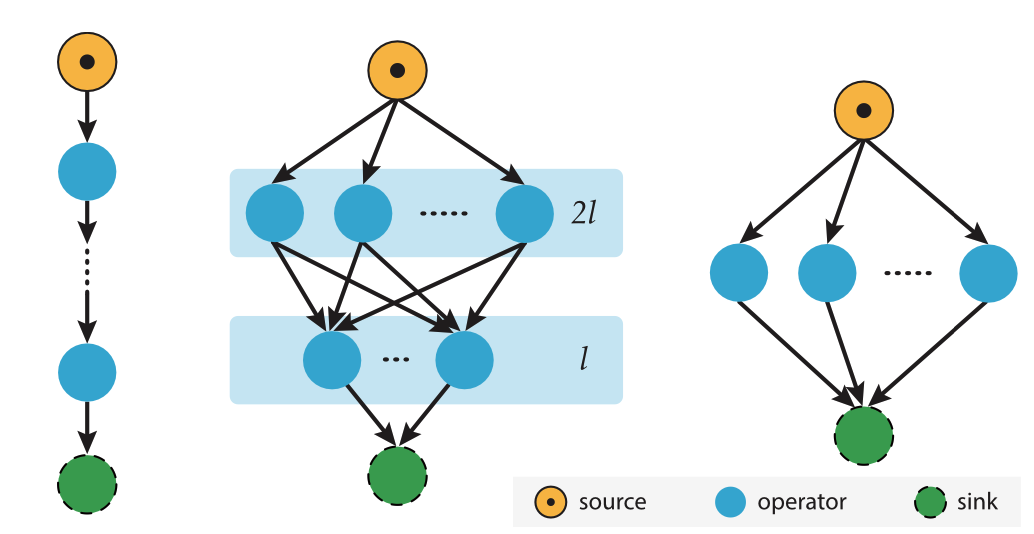
\includegraphics[width=0.9\linewidth]{res/topologies.png}
\captionof{figure}{Sequentielle, replizierte und Diamant-Topologie, Quelle: \cite{efficient-operator-placement}. }
\label{topologies}
\end{minipage}
\hspace{10pt}
\begin{minipage}{0.45\textwidth}
    In den dargestellten Topologien hat jede Schicht mindestens einen Operator. 
    Die erste und letzte Schicht verfügen jeweils über einen Operator, die Quelle und das Becken. 
    Alle Ressourcentopologien haben die gleiche Anzahl an Ressourcen.
\end{minipage}



\subsection{Experimentelle Ergebnisse}

Für das Experiment werden die Laufzeit (LZ) und die Qualitätseinbuße (QE) betrachtet \cite{efficient-operator-placement}.
Diese Merkmale werden mit der optimalen Lösung verglichen. $rt$ beschreibt die benötigte Zeit, 
um eine Lösung zu finden, pd beschreibt die Abweichung von der optimalen Lösung. 
Zusätzlich wird der Beschleunigungsfaktor (bf) definiert als $bf = rt_{optimal} / rt_i$, wobei $rt_i$ die Zeit für die Heuristik $i$ ist.
Le wird definiert als $le_i = \frac{F_i - F_{ODP}}{1 - F_{ODP}}$ \cite{efficient-operator-placement}, 
wobei $F_i$ die Zielfunktion der Heuristik $i$ ist.

Wie in \ref{OPP-Definition} definiert, werden im Experiment Verfügbarkeit, 
Netzwerklatenz und Antwortzeit als QoS selektiert und folglich mit der Straffunktion minimiert. 


% ODP definieren

Die Berechnung der Optimallösung weist eine effiziente Laufzeit für Diamant-Topologien auf. 
Diese Berechnung ist in unter einer Sekunde verfügbar. Bei replizierten und sequentiellen Topologien benötigt die Berechnung deutlich länger. 
Für replizierte Topologien dauert die Evaluation mehr als 8 Stunden (=32193 aus Tabelle). \\
\begin{table}[htbp]  
    \centering
    \caption{Evaluation der Heuristiken}
    \begin{tabular}{llllll}
    \toprule
    Methode                          &       & \textcolor{red}{Diamand}        & \textcolor{red}{Sequentiell}            & \textcolor{red}{Repliziert}                & Durchschnitt       \\
    \midrule
    ODP                              &LZ     &  0.1      & 41.4             & 915.2            &                  \\
                                     &LZ     &  0.8      & 2174.8           & 32193.9          &                  \\
    \cmidrule{1-5}
    Lokale Suche                     &BF     &  0.68     & 150.54           & 353.07           & 215.81           \\
                                     &QE     &0\%        & 1\%              &4\%               & 1\%              \\
    Tabusuche                       &BF      &  0.31     & 65.91            & 64.93            & 83.53            \\
                                     &QE     &0\%        & 1\%              &4\%               & 1\%              \\           
    Greedy First-Fit                 &BF     &  454.40   & $56 \cdot 10^4$  & $12 \cdot 10^6$  & $11 \cdot 10^6$  \\
                                     &QE     &0\%        & 7\%              &5\%               &11\%              \\
    Greedy First-Fit (keine $\delta$)&BF     &  454.40   & $56 \cdot 10^4$  & $12 \cdot 10^6$  & $11 \cdot 10^6$  \\
                                     &QE     &34\%       & 7\%              &24\%              & 19\%             \\
    \bottomrule
    \multicolumn{5}{l}{\footnotesize Tabelle aus des Experiments \cite{efficient-operator-placement}, \textcolor{red}{Vergleich für dre Topologien (Diamand, Sequentiell, Repliziert)}}\\
    \multicolumn{5}{l}{\footnotesize BF = Beschleunigungsfaktor, QE = Leistungseinbuße, LZ = Laufzeit}\\
    \end{tabular}
    \label{experiment-tabelle}
\end{table} 

Aus Tabelle \ref{experiment-tabelle} ist zu erkennen, dass Greedy First-Fit die schnellste Lösung bietet. 
Da die übrigen Heuristiken auf Greedy First-Fit basieren, entspricht das auch den Erwartungen. 
Trotz des hohen Beschleunigungsfaktors $bf$ liefern Greedy First-Fit und Greedy First-Fit (ohne $\delta$) degradierte Lösungen. 
Somit ergibt sich ein Kompromiss zwischen der Qualität der Lösung und der Laufzeit des Algorithmus. 
Auffällig ist die Diskrepanz zwischen der Greedy First-Fit Implementierung mit und ohne Straffunktion $\delta$. 
Bei Beschleunigungsfaktoren ähnlicher Größenordnung resultieren die verschiedenen Implementierungen 
in unterschiedlichen Qualitäten der Lösung, besonders bei Diamant- und replizierten Topologien.

Lokale Suche ist im Experiment schneller als Tabusuche, jedoch ist die Qualität der Lösung geringer. 
Somit bietet die Tabusuche die beste Operatorplatzierung, mit der längsten Laufzeit. 
Trotzdem stellt sich die Berechnung als viel effizienter heraus als die optimale Lösung. 
Während die Laufzeit der optimalen Lösung für replizierte Topologien mehr als 8 Stunden beträgt, benötigt die Tabus
uche 8,2 Minuten. 
Die lokale Suche findet in 1,5 Minuten eine Lösung. Dabei beträgt die Qualitätseinbuße bei beiden Methoden 1\%. 
In der Degradation der Performance ist bei der lokalen und der Tabusuche kein klarer Unterschied zu erkennen. 

Es gibt in diesem Experiment keinen Gewinner. Zwischen den Heuristiken gibt es Kompromisse zwischen Schnelligkeit und Genauigkeit. 

\section{Konklusion und Ausblick}In dieser Arbeit wurden mehrere Heuristiken vorgestellt, die das NP-schwere Problem der Operatorplatzierung approximieren.
Dabei handelt es sich um bekannte Methoden, die auch für andere NP-schwere Probleme genutzt werden. 
Mittels einer Straffunktion wurden die Heuristiken auf QoS-Attribute optimiert.\\
Die vorgestellten Heuristiken basieren auf dem Greedy First-Fit Ansatz und erweitern dessen Funktionalität durch Methoden wie lokale Suche und Tabusuche. 
Diese Heuristiken wurden in einem Experiment für drei verschiedene SVS-Architekturen evaluiert. 
Bei der Evaluation wurden sowohl die Laufzeit als auch die Qualität der Lösungen betrachtet. 
Es zeigte sich, dass keine der Heuristiken eine klare Überlegenheit aufweist. 
Beispielsweise führte die Greedy First-Fit Heuristik zu schnellen, jedoch qualitativ minderwertigen Lösungen, 
während die lokale Suche und die Tabusuche qualitativ bessere Platzierungen erreichten, jedoch mehr Zeit benötigten. 
Dennoch zeigten alle Heuristiken eine deutliche Verkürzung der Laufzeit im Vergleich zur Berechnung der optimalen Lösung.\\\\

Zukünftig werden wir komplexere Heuristiken entwickeln, die das OPP-Problem noch besser approximieren können. 
Die vorgestellten Methoden wurden zur Kompilierzeit verwendet, was bei dynamischen Veränderungen ineffizient ist. 
Deshalb wollen wir uns auf Heuristiken fokussieren, die zur Laufzeit angepasst werden können.
Zudem wollen wir die erneute Konfiguration während der Laufzeit analysieren, damit Big Data-Anwendungen auf verändernde Bedingungen reagieren können.

\newpage
\bibliography{biblio}

\end{document} 